\begin{figure}
\begin{center}
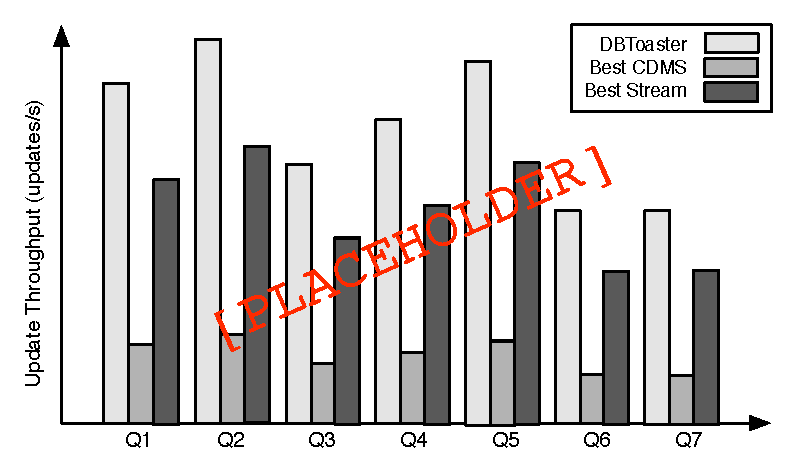
\includegraphics[width=3in]{../graphics-tmp/placeholder_bakeoff}
\end{center}
\label{fig:exp:bakeoff}
\caption{Comparison of DBToaster with the best performing commercial database and stream processor on each of the test queries}
\end{figure}

\begin{figure}
\begin{center}
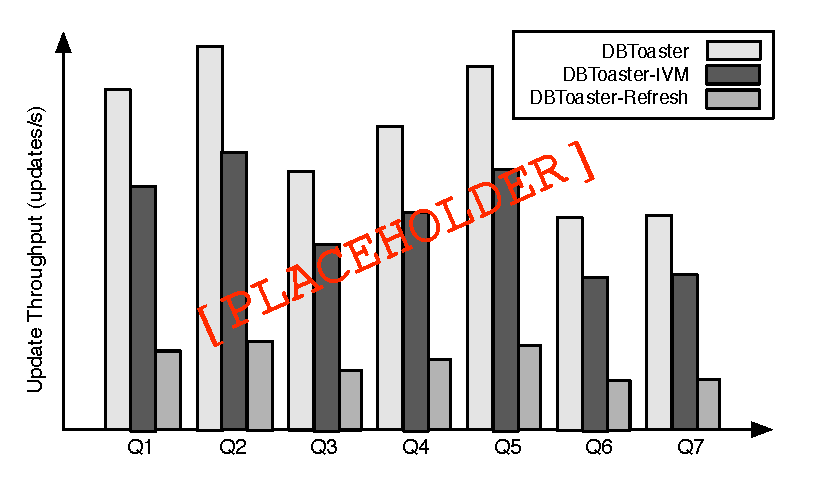
\includegraphics[width=3in]{../graphics-tmp/placeholder_throughput_all}
\end{center}
\label{fig:exp:bakeoff}
\caption{Comparison of DBToaster invoked with full recursive compilation, and with varying levels of depth restricted compilation.}
\end{figure}

\begin{figure}
\begin{center}
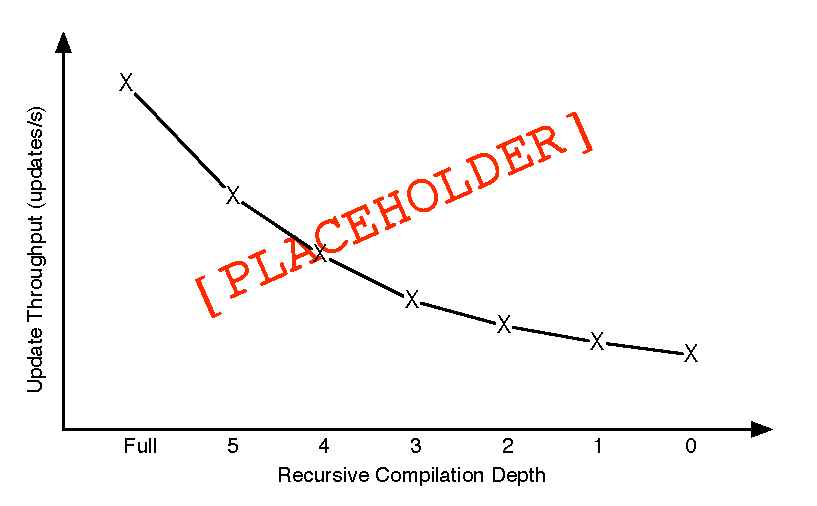
\includegraphics[width=3in]{../graphics-tmp/placeholder_throughput_ssb4}
\end{center}
\label{fig:exp:bakeoff}
\caption{Varying DBToaster's compile depth on a high-join width query.}
\end{figure}

\begin{figure}
\begin{center}
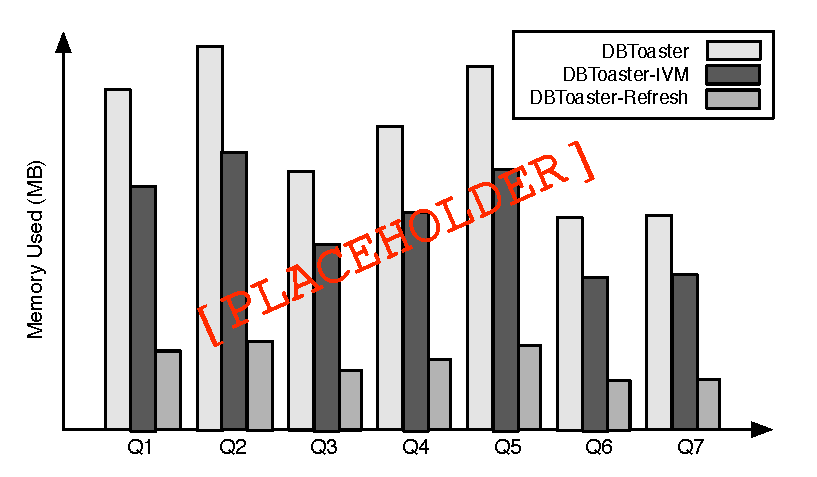
\includegraphics[width=3in]{../graphics-tmp/placeholder_memory_all}
\end{center}
\label{fig:exp:bakeoff}
\caption{Memory used by DBToaster for full recursive compilation and with varying levels of depth restricted compilation.}
\end{figure}


\begin{figure}
\begin{center}
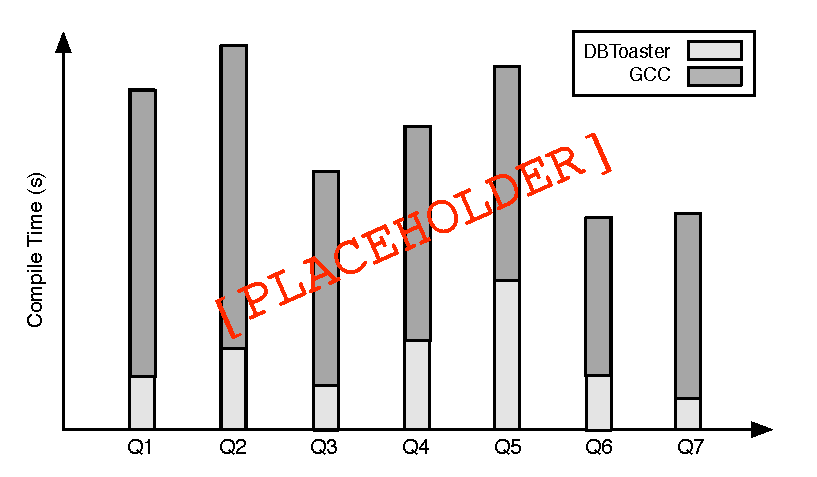
\includegraphics[width=3in]{../graphics-tmp/placeholder_compile_all}
\end{center}
\label{fig:exp:bakeoff}
\caption{Time taken by the DBToaster compiler to compile each of the test queries.}
\end{figure}